\chapter{Complex Numbers}
  \section{Complex Number I}
  \begin{figure}[H]
    \centering
    \includegraphics[page=145,width=\textwidth]{../Diagrams/Argand.pdf}
    \caption{\ref{source:complex-polar} The polar representation of a complex number.}
    \label{fig:complex-polar}
  \end{figure}
  \begin{stbox}{General Information}
    \begin{enumerate}
      \item Find the square root of \(x+iy\): Let \(\sqrt{x+iy}=a+bi\). Then square both sides \& solve.
      \item Simplifying fractions: multiply by the denominator's conjugate
      \[\frac{a+bi}{c+di}=\frac{a+bi}{c+di}\cdot\frac{c-di}{c-di}=\cdots.\]
      \item Polynomials:
      \begin{enumerate}
        \item Fundamental Theorem of Algebra: If \(p(z)\coloneq \sum_{i=0}^{n}a_iz^i\) is a polynomial of degree \(n \geq 1\) with complex coefficients, then there exists complex numbers \(c_i\) for each \(1 \leq i \leq n\) such that 
        \[p(z)=a_n \prod_{i=1}^{n}(z-c_i).\]
        \item If a polynomial in real coefficients only has root \(a+bi\), then \(a-bi\) is another root.
      \end{enumerate}
    \end{enumerate}
    \end{stbox}
        \begin{example}{}{}
          Find the roots of \(iz^2+2z+3i=0\).
          \begin{align*}
            z^2-2iz+3&=0\\
            z&=\frac{2i \pm \sqrt{(2i)^2-4(1)(3)}}{2(1)}=i \pm \frac{\sqrt{-16}}{2}=i \pm 2i
          \end{align*}
          So, \(z=3i\) or \(z=-i\).
        \end{example}
        \begin{example}{N2010/2/1}{}
          One root of the equation \(x^4+4x^3+ax+b=0\), where \(a\) and \(b\) are real, is \(x=-2+i\). Find the values of \(a\) and \(b\) and the other roots.\\[3mm]
          Substitute \(-2+i\) into the equation:
          \begin{align*}
            (-2+i)^4+4(-2+i)^3+(-2+i)^2+a(-2+i)+b&=0\\
            -12+16i&=2a-b-ai\\
            a=-16, &\hphantom{=}\ \ 2a-b=-12
          \end{align*}
          Therefore, \(a=-16\), \(b=-20\).\\[3mm]
          \emph{Since all the coefficients of the polynomial are real} (\textbf{explain}), \(-2-i\) is another root. Now, \(x^4+4x^3+ax+b=(x-(-2+i))(x-(-2-i))(cx+d)\) for some \(c,d \in \mathbb{R}\).\\[3mm]
          Accordingly, substitute \(x=0\), then \(x=2\), and solve. Alternatively, notice \(x^4+4x^3+ax+b=(x^2-2(-2)x+((-2)^2+1^2))(x^2+cx+d)=(x^2+4x+5)(x^2+4x+5)\). Either ways, we have \(c=0\) and \(d=-4\). As such, the last two roots are \(x=-2 \pm i\) and \(x=\pm 2\). 
        \end{example}
      \begin{stbox}{}
        \begin{itemize}[label=\hphantom{1.}]
          \item
          \begin{enumerate}[label=(\alph*)]
            \setcounter{enumi}{2}
            \item Simultaneous equations: Solve as usual.
            \item Properties of modulus: \(\lvert z_1^xz_2^y \rvert=\lvert z_1 \rvert^x \lvert z_2 \rvert^y\), for any \(x,y \in \mathbb{R}\).
            \item Properties of arguments (same as \(\log\)): \(\arg(z) \in (-\pi,\pi]\) and \(\arg(z_1^xz_2^y)=x\arg(z_1)+y\arg(z_2)\) for any \(x,y \in \mathbb{R}\).
            \item Polar form: \(z=re^{i\theta}\).
            \item Polar/Trigonometric form: \(z=r[\cos(\theta)+i\sin(\theta)]\).
          \end{enumerate}
        \end{itemize}
  \end{stbox}
  \begin{note}
    Show that the value of \(w^n\) is either \(2^n\) or \(2^{-n}\) for integers \(n\).\\[3mm]
    Then we \textbf{must} show that \(w^n=\cdots=\begin{cases}
      2^n(1)=2^n&\text{if }n\text{ even},\\
      2^n(-1)=-2^n&\text{if }n\text{ odd}.
    \end{cases}\) 
  \end{note}
  \begin{note}
    Common tricks to know:
    \begin{enumerate}
      \item Replace all occurrences of \(w\) in a polynomial \(P(x)\) with \(-w\).
      \item Notice that a geometric series is being used. E.g. \(\frac{1}{z^2}-\frac{1}{z}+1-z+z^2=\frac{z^5+1}{z^2(z+1)}\). 
    \end{enumerate}
  \end{note}
\section{Complex Numbers II}
\begin{theorem}{De Moivre's Theorem}{}
  Let \(z\) be a complex number, \(n\) an integer, and \(\theta\) an angle. Suppose \(z=re^{i\theta}\). Then, 
  \[z^n=r^ne^{in\theta}=r^n[\cos(n\theta)+i\sin{n\theta}].\]
\end{theorem}
\begin{stbox}{General Information}
  \begin{enumerate}
    \item All \(n\)th roots of any complex number are the same distance \(r\) from the origin and have the same angular separation, \(\pi/n\).
    \item Note that \(1+e^{i\theta}=e^{i\theta/2}(e^{-i\theta/2}+e^{i\theta/2})\).
    \item For \(z=re^{i\theta}\), we have \(z^n+z^{-n}=2\cos(n\theta)\) and \(z^n-z^{-n}=2i\sin(n\theta)\).
    \item The geometric meaning of multiplying by \(i\) is a anti-clockwise rotation by \(\pi\) radians.
    \item To represent roots of unity on an argand diagram, we should annotate 
    \begin{enumerate}
      \item The points representing the roots, as dots.
      \item The (dotted) circle which these points lie on.
      \item The radius of the circle.
      \item The angular separation between the roots.
    \end{enumerate}
    \begin{figure}[H]
      \centering
      \includegraphics[width=0.4\textwidth,page=2]{../Diagrams/Complex-revision.pdf}
      \caption{\ref{Me} Roots of unity on an argand diagram.}
      \label{fig:roots-of-unity}
    \end{figure}
    \item Loci (Use a \emph{compass})
    \begin{enumerate}
      \item The locus represented by \(\lvert z-a \rvert =r\) (or \(z=a+re^{i\theta}\)) is a \emph{circle} of radius \(r\) centered at \(A(x,y)\) (where \(a\coloneq x+iy\)).
      \begin{figure}[H]
        \centering
        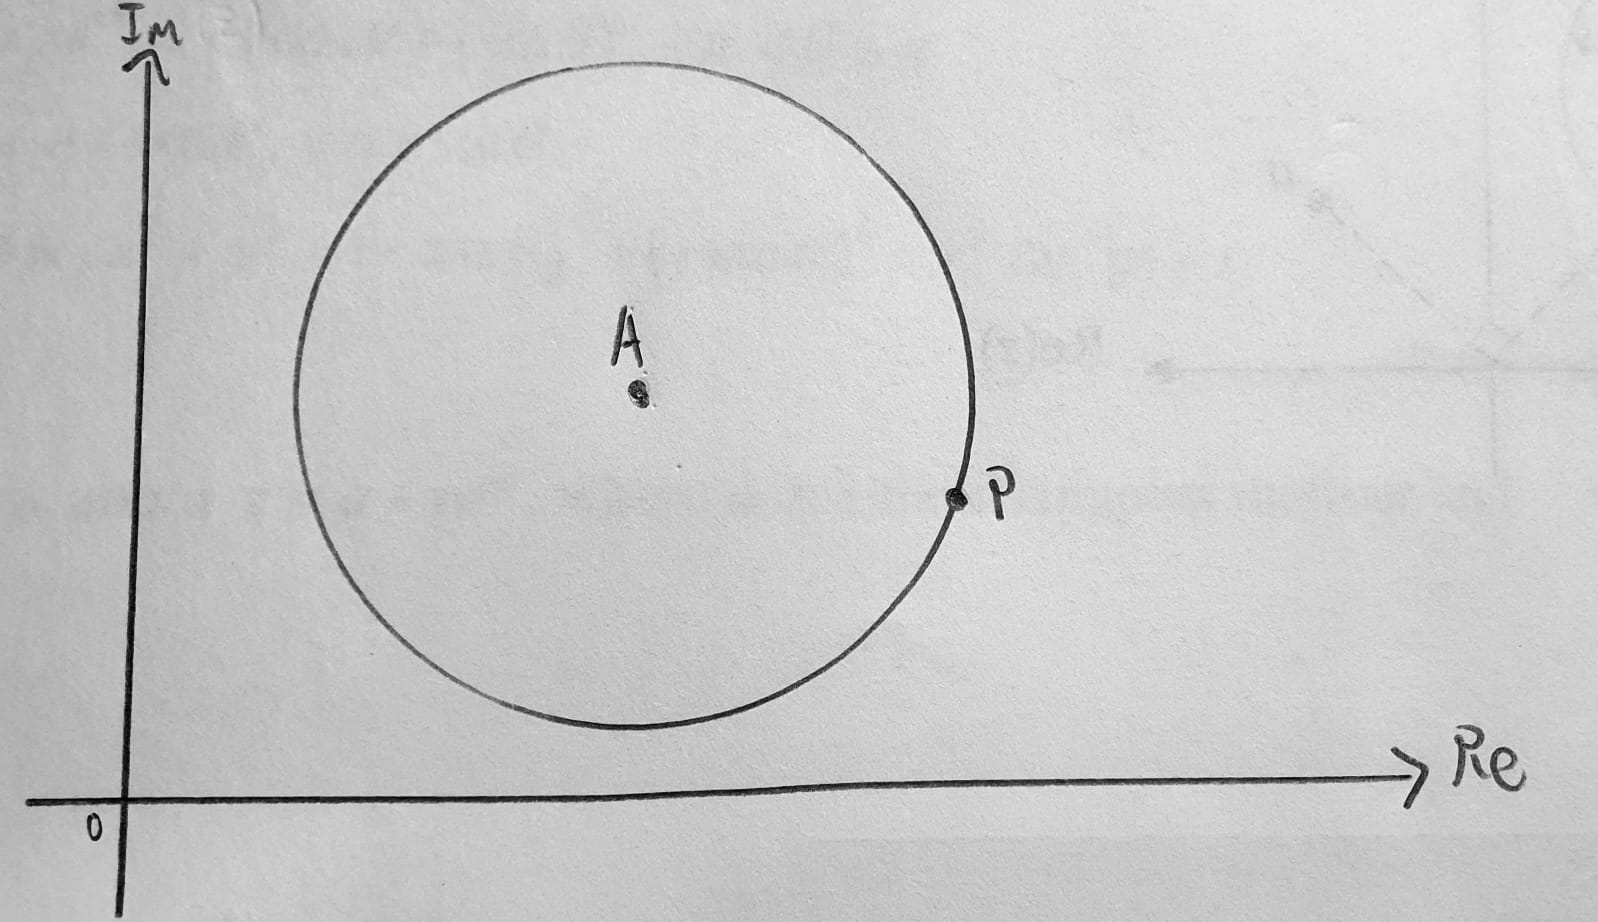
\includegraphics[scale=0.1]{../images/ComplexCircleLocus}
        \caption{\ref{Me} The locus of \(\lvert z-a \rvert =r\).}
        \label{fig:circle-locus}
      \end{figure}
      \begin{enumerate}
        \item Either label the four points to the direct North, South, East, West of the circle, or denote the radius clearly. 
        \item The line segment, representing the furthest distance from a point to a circle, always cuts through the circle's centre. So, the distance
        \[\text{OP}_{\text{max}}-\text{OP}_{\text{min}}=2\cdot\text{radius}.\]
        \item The line segments, from a point to a circle that produces the largest angle, are tangents to the circle.
        \begin{figure}[H]
          \centering
          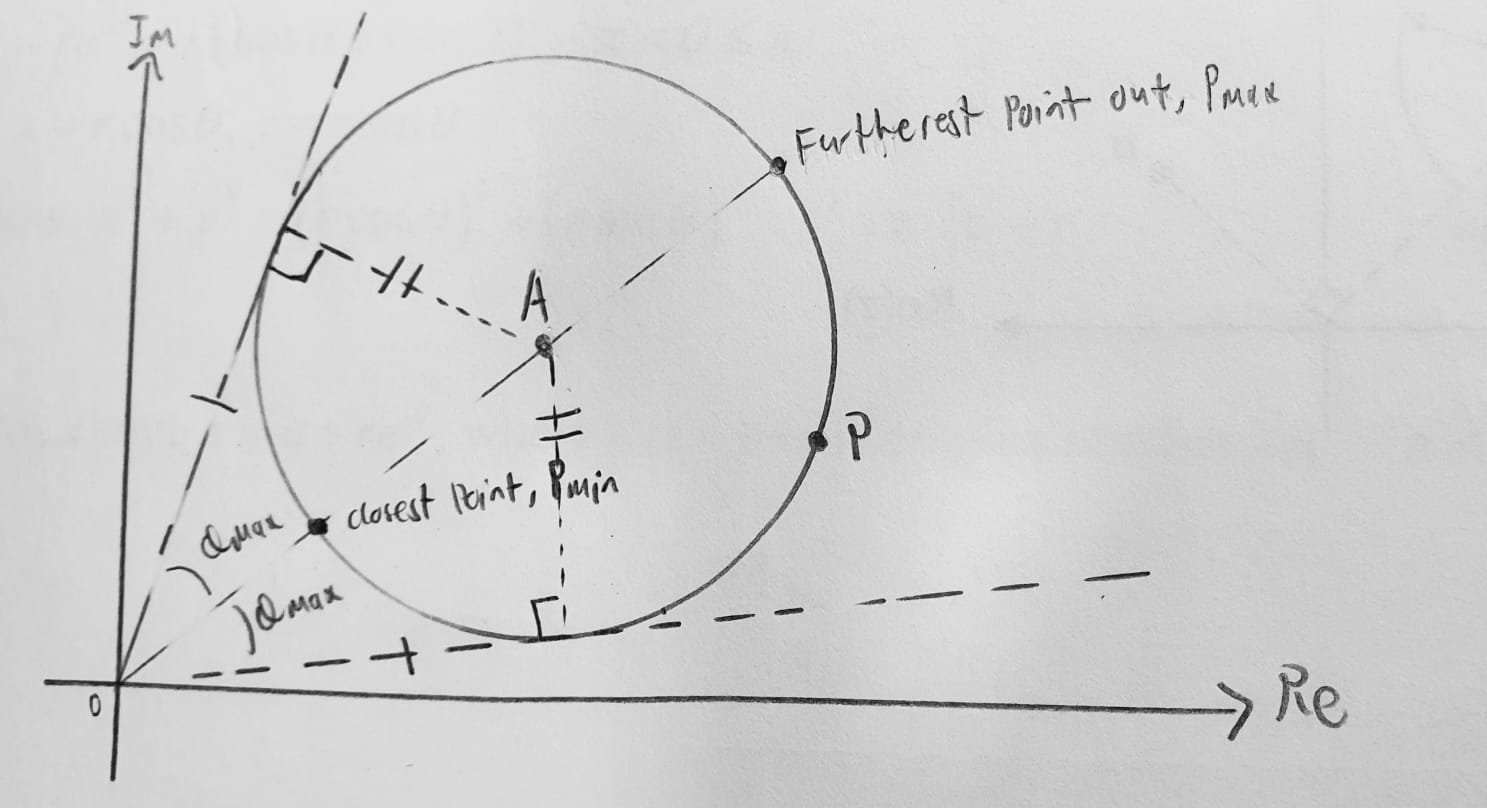
\includegraphics[scale=0.15]{ComplexLocusCircle-LargestAngleAndDistance.jpg}
          \caption{\ref{Me} Maxmium distance and angle of a point from a circle}
          \label{fig:locus-max-distance-and-angle-circle}
        \end{figure}
      \end{enumerate}
      \item The locus represented by \(\lvert z-a \rvert =\lvert z-b \rvert\) is the \emph{perpendicular bisector} of the line segment joining \(A\) and \(B\).
      \begin{figure}[H]
        \centering
        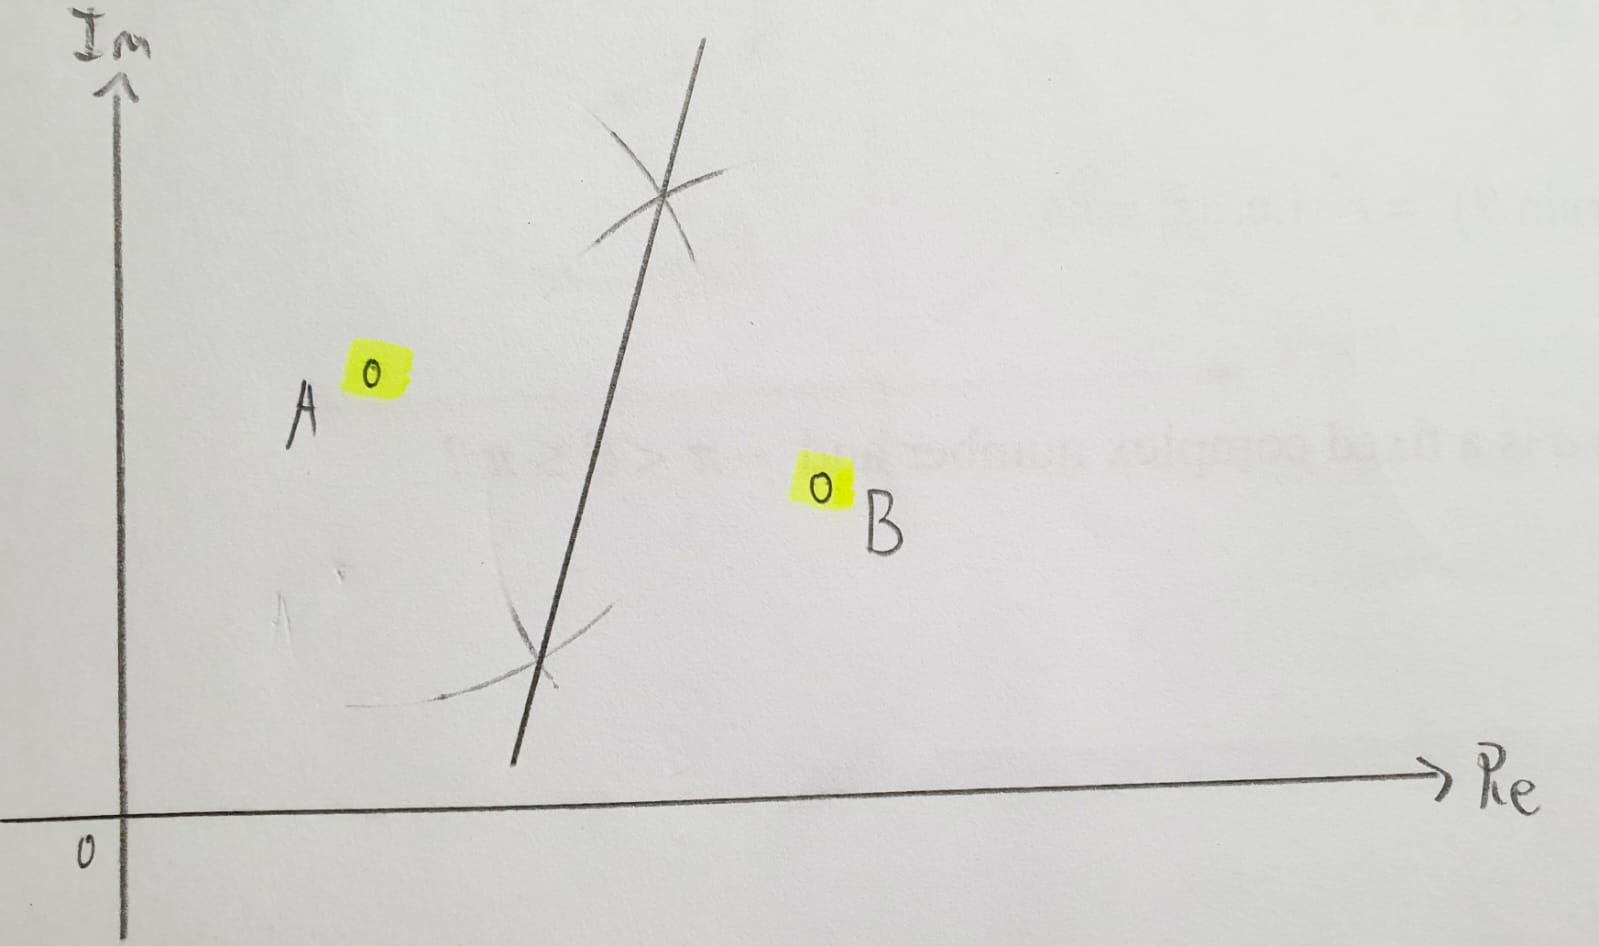
\includegraphics[scale=0.12]{../images/ComplexPerpendicularBisectorLocus}
        \caption{\ref{Me} The locus of \(\lvert z-a \rvert =\lvert z-b \rvert\), a perpendicular bisector.}
        \label{fig:perpendicular-bisector-locus}
      \end{figure}
      \item The locus represented by \(\arg(z-a)=\theta\) is the \emph{half-line} from \(A\) (excluding \(A\)) that makes an angle \(\theta\) with the \emph{positive} real axis.
      \begin{figure}[H]
        \centering
        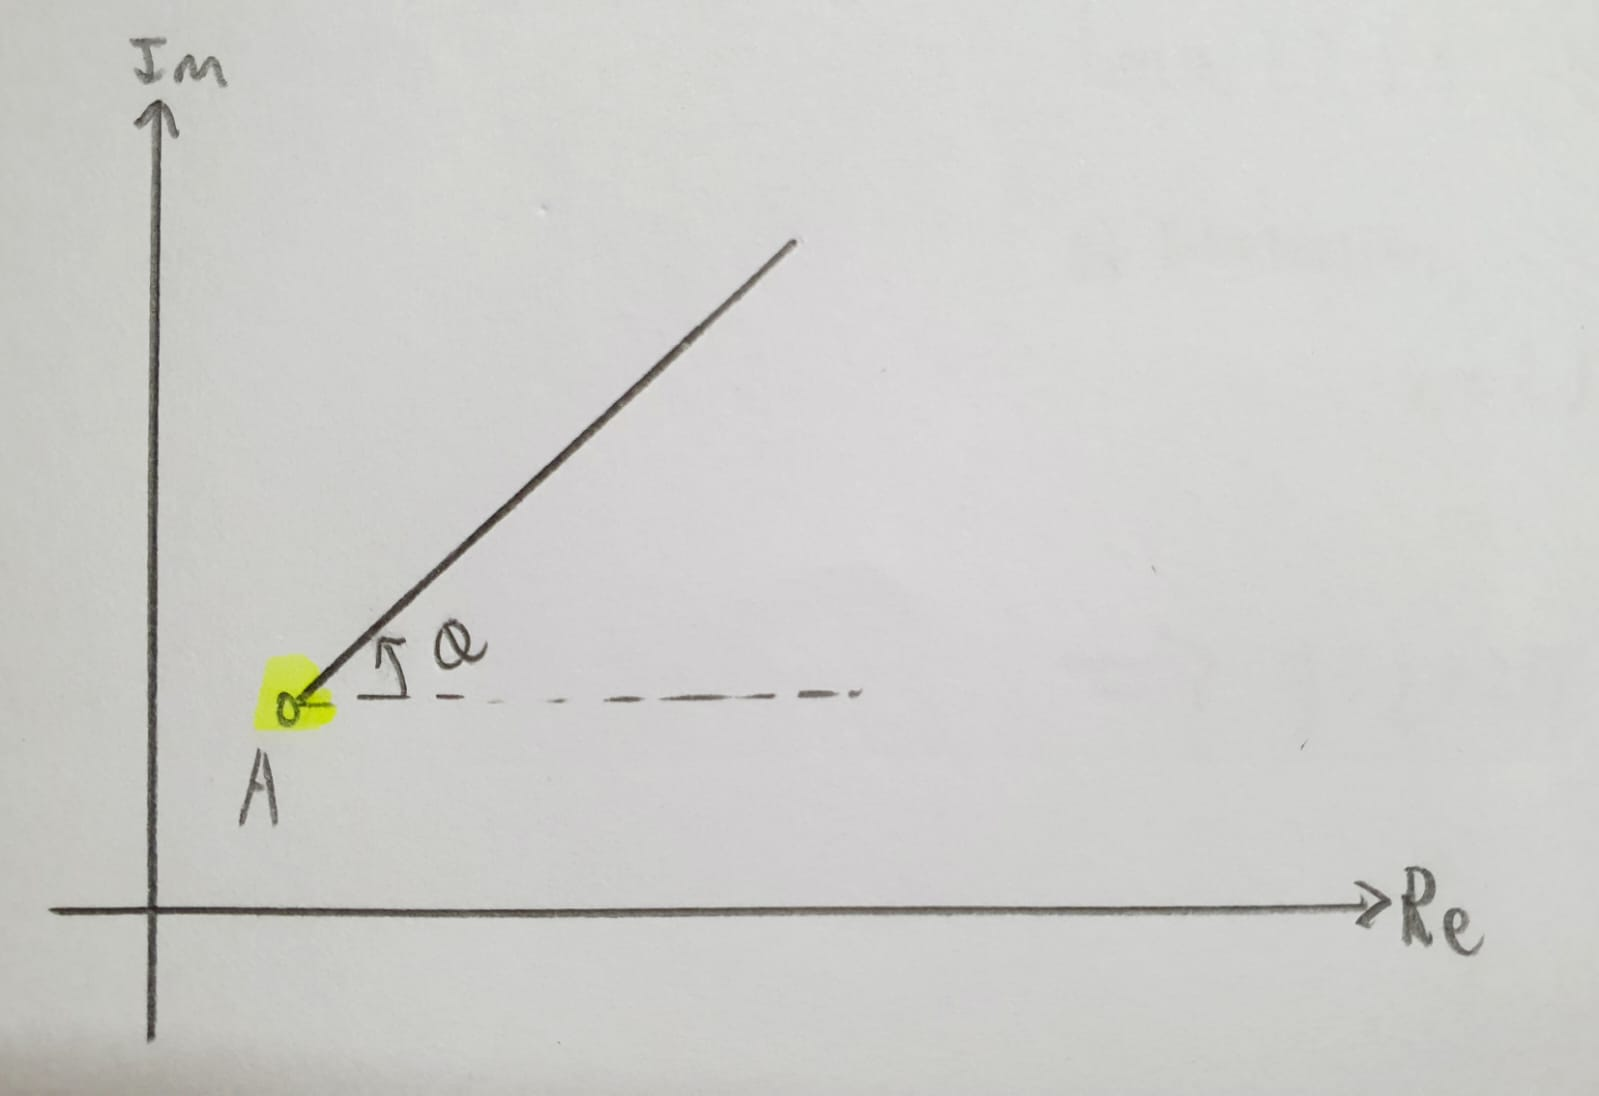
\includegraphics[scale=0.1]{../images/ComplexRotationByAngleTheta}
        \caption{\ref{Me} The locus of \(\arg(z-a)=\theta\), a half-line.}
        \label{fig:half-line-locus}
      \end{figure}
    \end{enumerate}
    \item There is no need to find the points of intersection between two loci, unless the questions states so. 
    \item Suppose we have a locus \(z\) represented by the predicate \(P(z)\). Then, for any \(a\in \mathbb{C}\), the locus of \(z+a\) is represented by \(P(z-a)\).
    \item Say we are given a locus \(z\) represented by \(\lvert z-a \rvert=r\), where \(a=\alpha+\beta i\). 
    \begin{enumerate}
      \item The greatest and least value of \(\lvert z \rvert\) are \(\lvert a \rvert \pm r\), respectively. 
      \item The greatest and least value of \(\arg(z)\) can be obtained geometrically, or by plotting 
      \[Y_1=\tan^{-1}\left(\frac{\beta\pm\sqrt{r^2-(X-\alpha)^2}}{X}\right)\]
      and finding the maximum/minimum point, respectively.
      \begin{figure}[H]
        \centering
        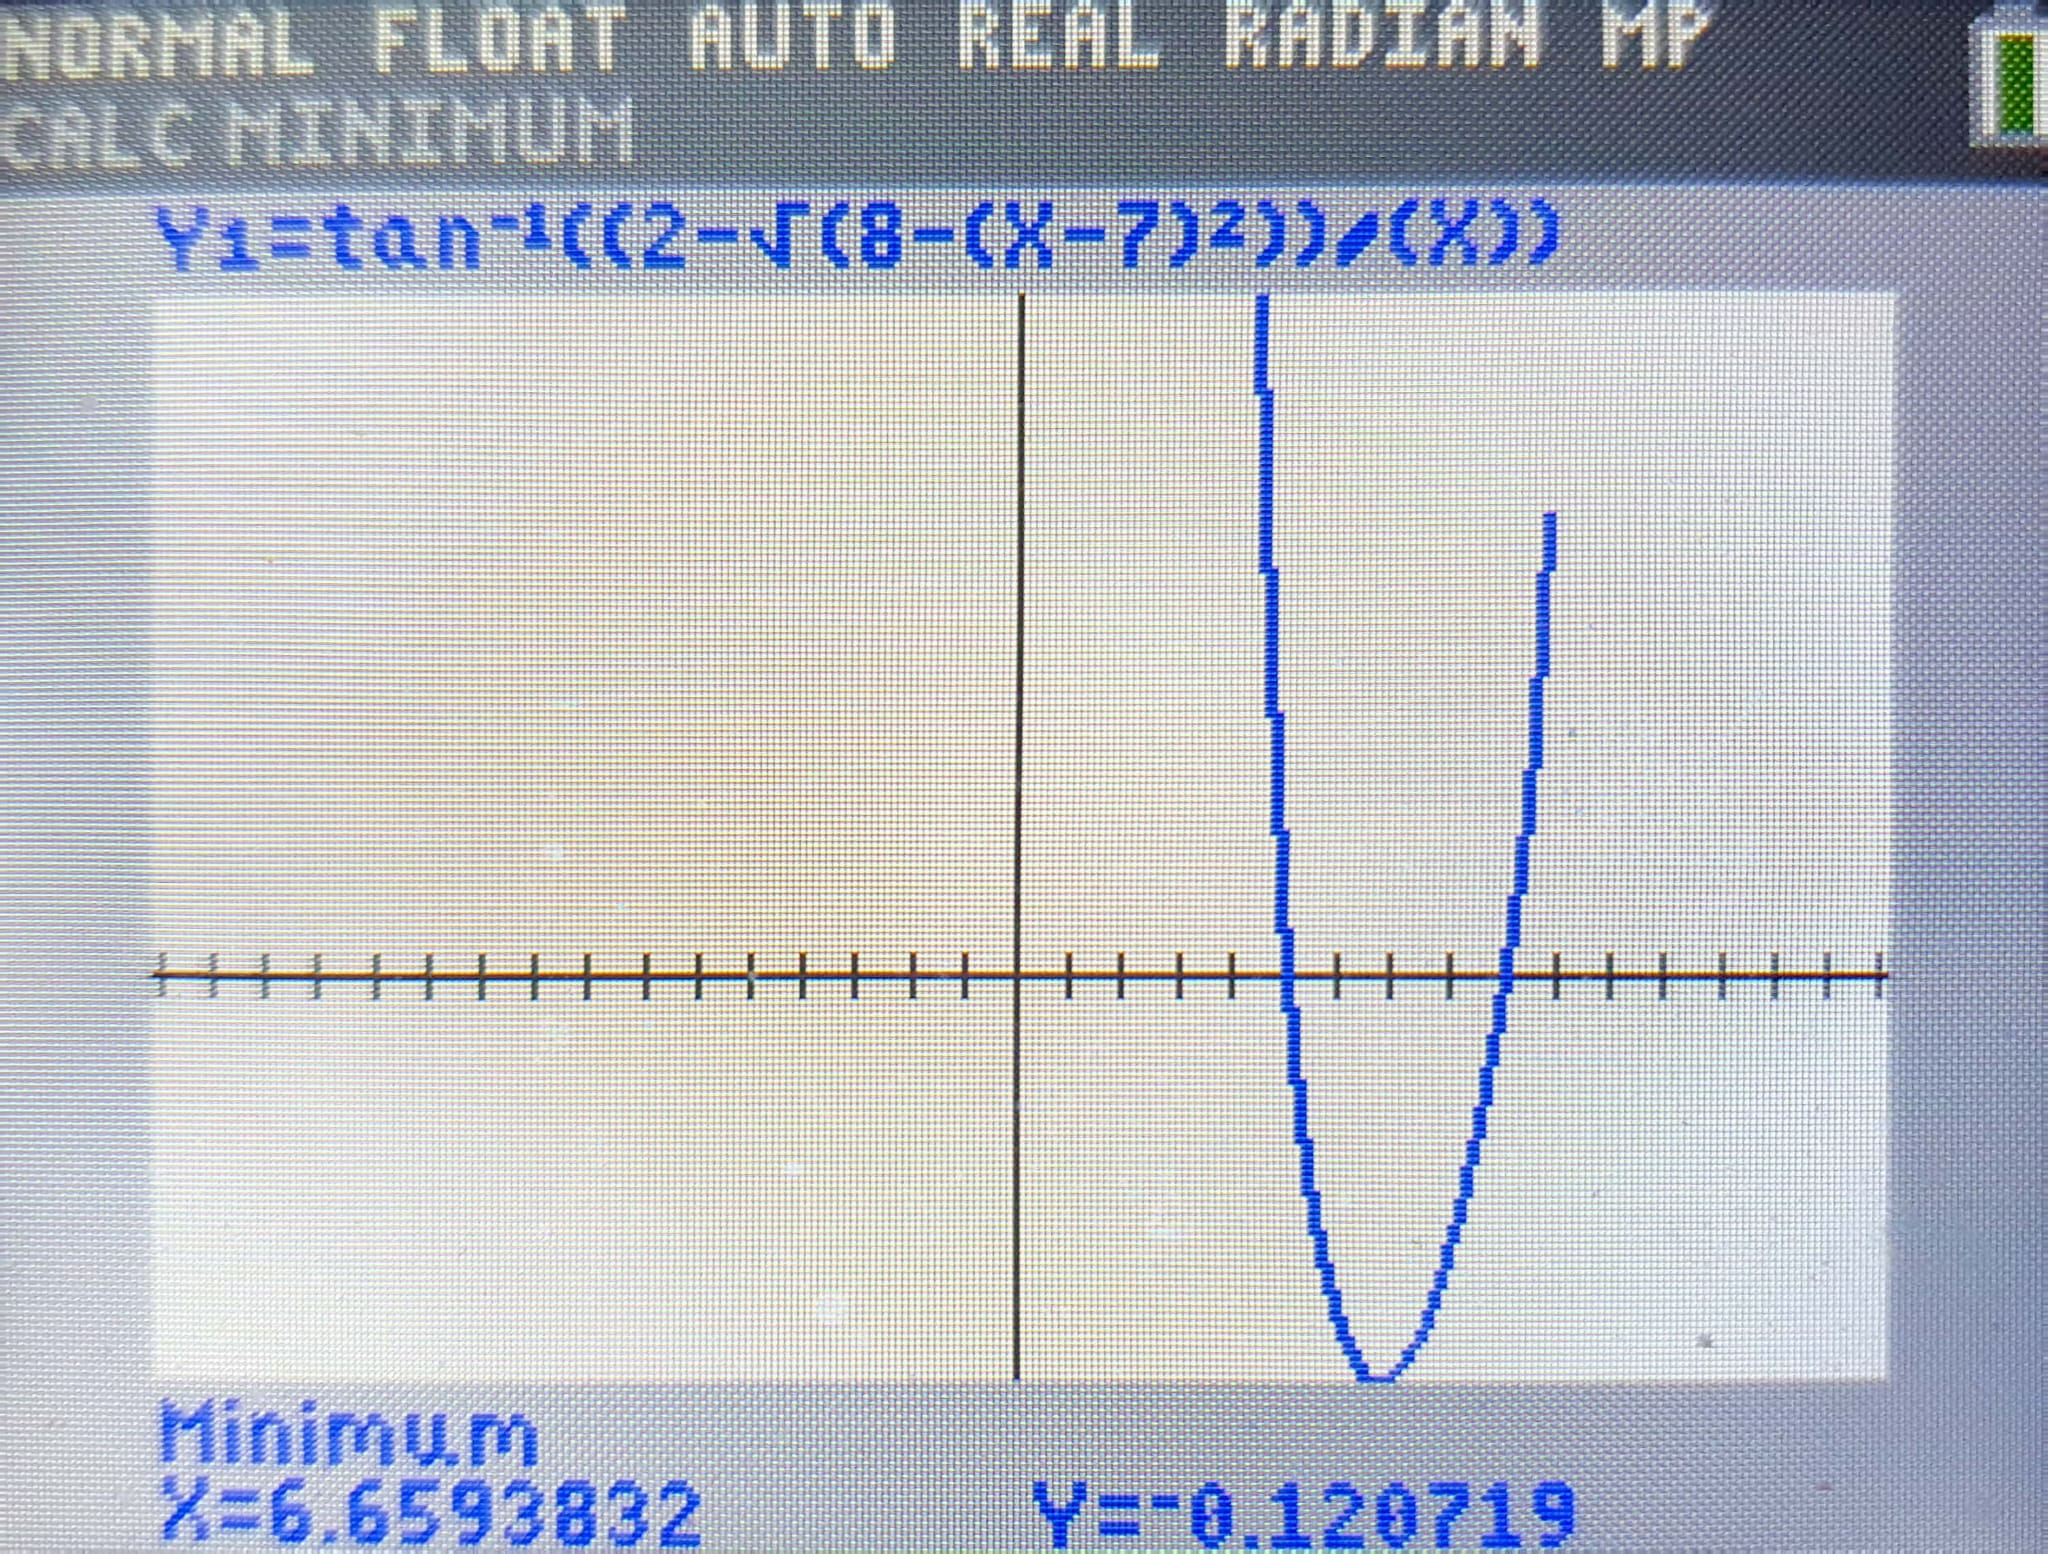
\includegraphics[width=0.5\textwidth]{../images/Complex-Numbers-My-Funnei-Technique.jpg}
        \caption{Brute force technique for finding maximum/minimum angles.}
        \label{fig:brute-force-complex}
      \end{figure}
    \end{enumerate}
  \end{enumerate}
\end{stbox}
\begin{note}
  To show that a \emph{half}-line \(\arg(z-a-bi)=\theta\) meets another loci \(L\), we need to show that 
  \begin{enumerate}[label=(\alph*)]
    \item The line \(y-b=\tan(\theta)(x-a)\) meets the loci \(L\) at some \((u,v)\).
    \item 
    \(\begin{cases}
      u>a &\text{if }\theta\in(-\pi/2,\pi/2),\\
      u=a &\text{if }\theta=\pm\pi/2,\\
      u<a &\text{if }\theta\in(\pi/2,\pi)\cup(-\pi,-\pi/2).
    \end{cases}\)
    \item  
    \(\begin{cases}
      v>b &\text{if }\theta\in(0,\pi),\\
      v=b &\text{if \(\theta=0\) or \(\theta=\pi\)},\\
      v<b &\text{if }\theta\in(-\pi,0).
    \end{cases}\)
  \end{enumerate}
  The latter two conditions must be shown to be clearly satisfied, to illustrate our understanding of \emph{half}-lines. For example, we may write
  \[x=\frac{2-\sqrt{3}}{4}\highlight[yellow]{>-2} \qquad y=\frac{1+10\sqrt{3}}{4}\highlight[yellow]{>1}.\]
\end{note}
\begin{example}{TQ 10(b)}{}
  Show that \(\cot^2(2\pi/5)\) is a root of the equation \(px^2+qx+r=0\), where we are given 
  \[\cot(4\theta)=\frac{\cot^4(\theta)-6\cot^2(\theta)+1}{4\cot^3(\theta)-4\cot(\theta)}.\]
  \rule{20cm-137.0549pt}{0.05mm}
  First notice that \(\cot(8\pi/5)=-\cot(2\pi/5)\). So, 
  \[-\cot(2\pi/5)=\frac{\cot^4(2\pi/5)-6\cot^2(2\pi/5)+1}{4\cot^3(2\pi/5)-4\cot(2\pi/5)}.\]
  Simplifying gives 
  \[5[\cot^2(2\pi/5)]^2-10[\cot^2(2\pi/5)]+1=0.\]
  Thus, \(x=\cot^2(2\pi/5)\) is a root of the equation \(5x^2-10x+1=0\). 
\end{example}
\begin{example}{RV FM 2023 J2 CT}{}
  Show, by using De Moivre's theorem, that provided \(\cos(\theta)\neq 0\), 
  \[\sum_{k=1}^{12}{(-1)^{k-1}\cos((2k-1)\theta)}=\frac{\sin^2(P\theta)}{\cos(\theta)}\]
  where \(P\) is a constant to be determined.

  \rule{20cm-137.0549pt}{0.05mm}

  Let \(C=\sum_{k=1}^{12}{(-1)^{k-1}\cos((2k-1)\theta)}\) and \(S=\sum_{k=1}^{12}{(-1)^{k-1}\sin((2k-1)\theta)}\). Then, for \(z=e^{i\theta}\),
  \begin{align*}
    C+iS &=\sum_{k=1}^{12}{(-1)^{k-1}[\cos((2k-1)\theta)+i\sin((2k-1)\theta)]}\\
    &=\sum_{k=1}^{12}{z(-z^2)^{k-1}}\\
    &=\frac{z\left(1-(-z^2)^{12}\right)}{1-(-z^2)}\\
    &\vdotswithin{=}\\
    &=\frac{-ie^{i(12\theta)}\sin(12\theta)}{\cos(\theta)}.
  \end{align*}
  So, comparing real parts,
  \[C=\frac{(-i)\cdot i\sin(12\theta) \cdot \sin(12\theta)}{\cos(\theta)}=\frac{\sin^2(12\theta)}{\cos(\theta)}.\]
\end{example}
\begin{note}
  Algebraic tricks to know.
  \begin{enumerate}
    \item Factoring out \(e^{i\theta/2}\), given an expression involving \(e^{i\theta}\), can help in simplifying expressions.
    \item Let \(r_1,\dots,r_n\) be the roots of the polynomial \(p(z)\coloneq\sum{a_iz^i}\). To find the sum or product of the roots, consider
    \begin{enumerate*}[itemjoin={, or\ }]
      \item Vieta's Formula
      \item comparing the coefficients of \(p(z)=\highlight[yellow]{a_n}(z-r_1)(z-r_2)\cdots(z-r_n)\).
    \end{enumerate*}
    \item[\(\bigstar\)] Take extra caution to note whether a geometric progression is present.
    \item Let \(n\in \mathbb{Z}^{+}\). Suppose that \(n\) is odd, and we want to express \(\sin^n(\theta)\) as a linear combination of \(\sin(m\theta)\), for \(m\in \mathbb{Z}^{+}\). First notice that \(z^k-\frac{1}{z^k}=2i\sin(k\theta)\), for \(z=e^{i\theta}\). Then, use this fact in conjunction with the binomial theorem:
    \begin{align*}
      \left( z-\frac{1}{z} \right)^n &= \sum_{k=0}^{n}{\binom{n}{k}(-1)^kz^{n-2k}}\\
      [2i\sin(\theta)]^n &= \sum_{k=0}^{\lfloor n/2 \rfloor}{\binom{n}{n-2k}\left( z^{n-2k}-\frac{1}{z^{n-2k}} \right)}.
      % \binom{n}{n}\left( z^n-\frac{1}{z^n} \right)+\binom{n}{n-1}\left( z^{n-2}-\frac{1}{z^{n-2}} \right)+\dots+\binom{n}{\lfloor n/2 \rfloor}\left( z-\frac{1}{z} \right)\\
    \end{align*}
    Comparing imaginary parts, we get \(\sin^n(\theta)\) in the desired form:
    \[\sin^n(\theta)=\frac{1}{2^{n-1}}
    % \left[ \sin(n\theta)+\binom{n}{n-2}\sin((n-2)\theta)+\dots+\binom{n}{\lfloor n/2 \rfloor}\sin(\theta) \right]
    \sum_{k=0}^{\lfloor n/2 \rfloor}{\binom{n}{n-2k}\sin((n-2k)\theta)}.\]
    (Similarly, we can express \(\cos^n(\theta)\) as a linear combination of \(\cos(m\theta)\).)
    \item Now, consider even \(n\), instead. Then, recall that \(z^k+\frac{1}{z^k}=2\cos(k\theta)\). As such,
    \begin{align*}
      [2i\sin(\theta)]^n &= \sum_{k=0}^{n/2}{\binom{n}{n-2k}\left( z^{n-2k}-\frac{1}{z^{n-2k}} \right)}\\
      \sin^n(\theta) &= \frac{1}{2^{n-1}}\sum_{k=0}^{n/2}{\binom{n}{n-2k}\cos((n-2k)\theta)}.
    \end{align*}
    (The case for \(\cos^n(\theta)\) is again similar.)
    % \item Alternatively, we may be asked to express \(\sin(n\theta)\) as a linear combination of \(\sin(m\theta)\), using just De Moivre's theorem. Letting \(c\coloneq\cos(\theta)\) and \(s\coloneq\sin(\theta)\), we first expand
    % \begin{align*}
    %   \cos(n\theta)+i\sin(n\theta) &= [\cos(\theta)+i\sin(\theta)]^n\\
    %   &= \sum_{k=0}^{n}{\binom{n}{k}c^{n-k}i^{k}s^{k}}.
    % \end{align*}
    % Then, compare imaginary parts. (Or real parts, for \(\cos(n\theta)\).)
    \item Let \(n\in \mathbb{Z}^{+}\). Similarly, to find \(\sin(n\theta)\) in terms of powers of \(\sin(\theta)\), first apply De Moivre's theorem:
    \[\cos(n\theta)+i\sin(n\theta)=(c+is)^n=\sum_{k=0}^{n}{\binom{n}{k}c^{n-k}i^ks^k}.\]
    Then, we compare imaginary parts. (Or real parts, for \(\cos(n\theta)\).)
    \item Trigonometric identities:
    \begin{table}[H]
      \centering
      \begin{tabular}{M{0.3\textwidth}M{0.3\textwidth}}
        \toprule
        \(\pi-\theta\) & \(\pi/2-\theta\)\\
        \midrule 
        \(\begin{aligned}
          \sin(\pi-\theta)&=\sin(\theta)\\
          \cos(\pi-\theta)&=-\cos(\theta)\\
          \tan(\pi-\theta)&=-\tan(\theta)
        \end{aligned}\)
        % \begin{itemize}
        %   \item \(\sin(\pi-\theta)=\sin(\theta)\)
        %   \item \(\cos(\pi-\theta)=-\cos(\theta)\) 
        %   \item \(\tan(\pi-\theta)=-\tan(\theta)\)
        % \end{itemize}
        &
        \(\begin{aligned}
          \sin(\pi/2-\theta)&=\cos(\theta)\\
          \cos(\pi/2-\theta)&=\sin(\theta)\\
          \tan(\pi/2-\theta)&=\cot(\theta)
        \end{aligned}\)\\
        % \begin{itemize}
        %   \item \(\sin(\pi/2-\theta)=\cos(\theta)\)
        %   \item \(\cos(\pi/2-\theta)=\sin(\theta)\)
        %   \item \(\tan(\pi/2-\theta)=\cot(\theta)\)
        % \end{itemize}\\
        \bottomrule
      \end{tabular}
      \caption{}
      \label{table:trigonometric-identities}
    \end{table}
    \item Let \(z^n=1\). Then, \(\sum{z^i}=z^n\sum{z^i}=\sum{z^{n+i}}\).
    \item When asked to prove an identity involving binomial coefficients \(\binom{n}{k}\), try to factor the given form using the binomial theorem. 
  \end{enumerate}
\end{note}
\begin{example}{Algebraic tricks to know}{}
  \begin{enumerate}
    \item[1(a).] Simplifying a complex number \(w\) to a given form. 
    \begin{align*}
      w&=\frac{-ie^{2ki\pi/5}}{1-e^{2ki\pi/5}}=\frac{-ie^{2ki\pi/5}}{e^{ki\pi/5}\left[ e^{-ki\pi/5}-e^{ki\pi/5} \right]}=\frac{-ie^{ki\pi/5}}{-2i\sin(k\pi/5)}\\
      &=\frac{\cos(k\pi/5)+i\sin(k\pi/5)}{2\sin(k\pi/5)}=\frac{1}{2}[\cot(k\pi/5)+i]
    \end{align*}
    \item[1(b).]
    \[z=2\left( 1+e^{2ki\pi/3} \right)=2e^{ki\pi/3}\left( e^{-ki\pi/3}+e^{ki\pi/3} \right)=4\cos(k\pi/3)e^{ki\pi/3}.\]
    \item[1(c).] Let \(z_k=e^{2ki\pi/n}\) for all \(1\leq k\leq n\). In the case where \(n\) is odd, i.e. \(n=2m+1\), evaluate the series \(\sum_{k=1}^{n}{2(1+z_k)^{-1}}\).
    \begin{align*}
      \sum_{k=1}^{n}{\frac{2}{1+z_k}}&=\sum_{k=1}^{n}{\frac{2}{1+e^{2ki\pi/n}}}=\sum_{k=1}^{n}{\frac{2}{e^{ki\pi/n}\left( e^{-ki\pi/n}+e^{ki\pi/n} \right)}}=\sum_{k=1}^{n}{\frac{2e^{-ki\pi/n}}{2\cos(k\pi/n)}}\\
      &=\sum{k=1}^{n}\frac{\cos(k\pi/n)-i\sin(k\pi/n)}{\cos(k\pi/n)}=\sum_{k=1}^{n}{1-i\tan(k\pi/n)}\\
      &=n-i\Bigl[\bigl[\tan(\pi/n)+\tan((n-1)\pi/n)\bigr]+\bigl[\tan(2\pi/n)+\tan((n-2)\pi/n)\bigr]+...\\
      &\hphantom{={}}+\bigl[\tan(m\pi/n)+\tan((n-m)\pi/n)\bigr]+\tan(\pi)\Bigr]\\
      &=n+i(0+0+\dots+0)=n
    \end{align*}
    because \(\tan(\pi-\theta)=-\tan(\theta)\).
    \item[2.] We found that the roots of \((1+z)^4+(1-z)^4=0\) has roots \(i\tan(k\pi/8)\), where \(k=1,3,4,7\). Then, we were tasked to find the value of \(\tan^2(\pi/8)+\tan^2(3\pi/8)\) and \(\tan^2(5\pi/8)\tan^2(\pi/8)\tan^2(3\pi/8)\).\\[\baselineskip]
    Since \(\tan(\pi/8)=-\tan(7\pi/8)\) and \(\tan(3\pi/8)=-\tan(5\pi/8)\),
    \begin{align*}
      (1+z)^4+(1-z)^4 &= \highlight[yellow]{2}[z-i\tan(\pi/8)][z+i\tan(\pi/8)][z-i\tan(3\pi/8)][z+i\tan(3\pi/8)]\\
      &= \highlight[yellow]{2}[z^2+\tan^2(\pi/8)][z^2+\tan^2(3\pi/8)].
    \end{align*}
    Comparing constants/coefficients of \(z^2\), we obtain 
    \[\tan^2(\pi/8)\tan^2(3\pi/8)=1 \qquad\text{and}\qquad \tan^2(\pi/8)+\tan^2(3\pi/8)=6,\]
    respectively.  
    \item[3.] The case of \(n=5\): expressing \(\sin^5(\theta)\), in terms of \(\sin(m\theta)\).
    \begin{align*}
      \left( z-\frac{1}{z} \right)^5 &= z^5-5z^3+10z-\frac{10}{z}+\frac{5}{z^3}-\frac{1}{z^5}\\
      [2i\sin(\theta)]^5 &= \left( z^5-\frac{1}{z^5} \right)-5\left( z^3-\frac{1}{z^3} \right)+10\left( z-\frac{1}{z} \right)\\
      32i\sin^5(\theta) &= 2\sin(5\theta)-5(2)i\sin(3\theta)+10(2)i\sin(\theta)\\
      \sin^5(\theta) &= \frac{1}{16}\sin(5\theta)-\frac{5}{16}\sin(3\theta)+\frac{5}{8}\sin(\theta).
    \end{align*}
    \setcounter{enumi}{6}
    \item Let \(\omega=e^{2i\pi/11}\). We define
    \[\alpha=\omega+\omega^3+\omega^4+\omega^5+\omega^9 \qquad\text{and}\qquad \beta=\omega^{-1}+\omega^{-3}+\omega^{-4}+\omega^{-5}+\omega^{-9}.\]
    Find \((x-\alpha)(x-\beta)\) in its simplest form. Notice that \(\beta=\omega^{11}\beta=\omega^{10}+\omega^8+\omega^7+\omega^6+\omega^2\). As such,
    \[\alpha+\beta=\sum_{k=1}^{10}{\omega^k}=-1 \qquad\text{and}\qquad \alpha\beta=\underbrace{5+2\left( \sum_{k=1}^{10}{\omega^k} \right)}_{\text{the usual expansion}}=5-2=3.\]
    Now, \((x-\alpha)(x-\beta)=x^2-(\alpha+\beta)x+\alpha\beta=x^2+x+3\).
    \item Let 
    \begin{align*}
      C&=1-\binom{2n}{1}\cos(\theta)+\binom{2n}{2}\cos(2\theta)-\binom{2n}{3}\cos(3\theta)+\dots+\cos(2n\theta)\\
      S&=-\binom{2n}{1}\sin(\theta)+\binom{2n}{2}\sin(2\theta)-\binom{2n}{3}\sin(3\theta)+\dots+\sin(2n\theta),
    \end{align*}
    where \(n\) is a positive integer. Then, 
    \begin{align*}
      C+iS&=\sum_{r=0}^{2n}{(-1)^r\binom{2n}{r}[\cos(r\theta)+i\sin(r\theta)]}\\
      &=\sum_{r=0}^{2n}{\binom{2n}{r}(-1)^re^{i(r\theta)}}=\sum_{r=0}^{2n}{\binom{2n}{r}(1)^{2n-r}\left( -e^{i\theta} \right)^r}\\
      &=\left(1-e^{i\theta}\right)^{2n}=\left( e^{i\theta/2} \right)^{2n}\left( e^{-i\theta/2}-e^{i\theta/2} \right)^{2n}\\
      &=e^{in\theta}[-2i\sin(\theta/2)]^{2n}\\
      &=(-4)[\cos(n\theta)+i\sin(n\theta)]\sin^{2n}(\theta/2).
    \end{align*}
    Comparing real and imaginary parts,
    \[C=(-4)^n\cos(n\theta)\sin^{2n}(\theta/2) \qquad\text{and}\qquad S=(-4)^n\sin(n\theta)\sin^{2n}(\theta/2).\]
  \end{enumerate}
\end{example}
\begin{note}
  Geometrical tricks to know.
  \begin{enumerate}
    \item Where clarity may otherwise be lacking, consider making a line segment \emph{thicker} and \emph{label} it with ``\textrightarrow\ required points'' --- to indicate that it is the locus being requested for.  
    \item Be aware of any triangles, congruent triangles, common angles, and sides of common length. In particular, when a triangle has an angle of \(\pi/4=45^{\circ}\), it is an isosceles triangle. These observations are especially helpful in finding circle-line intersections.
  \end{enumerate}
\end{note}
\begin{example}{}{}
  \begin{figure}[H]
    \centering
    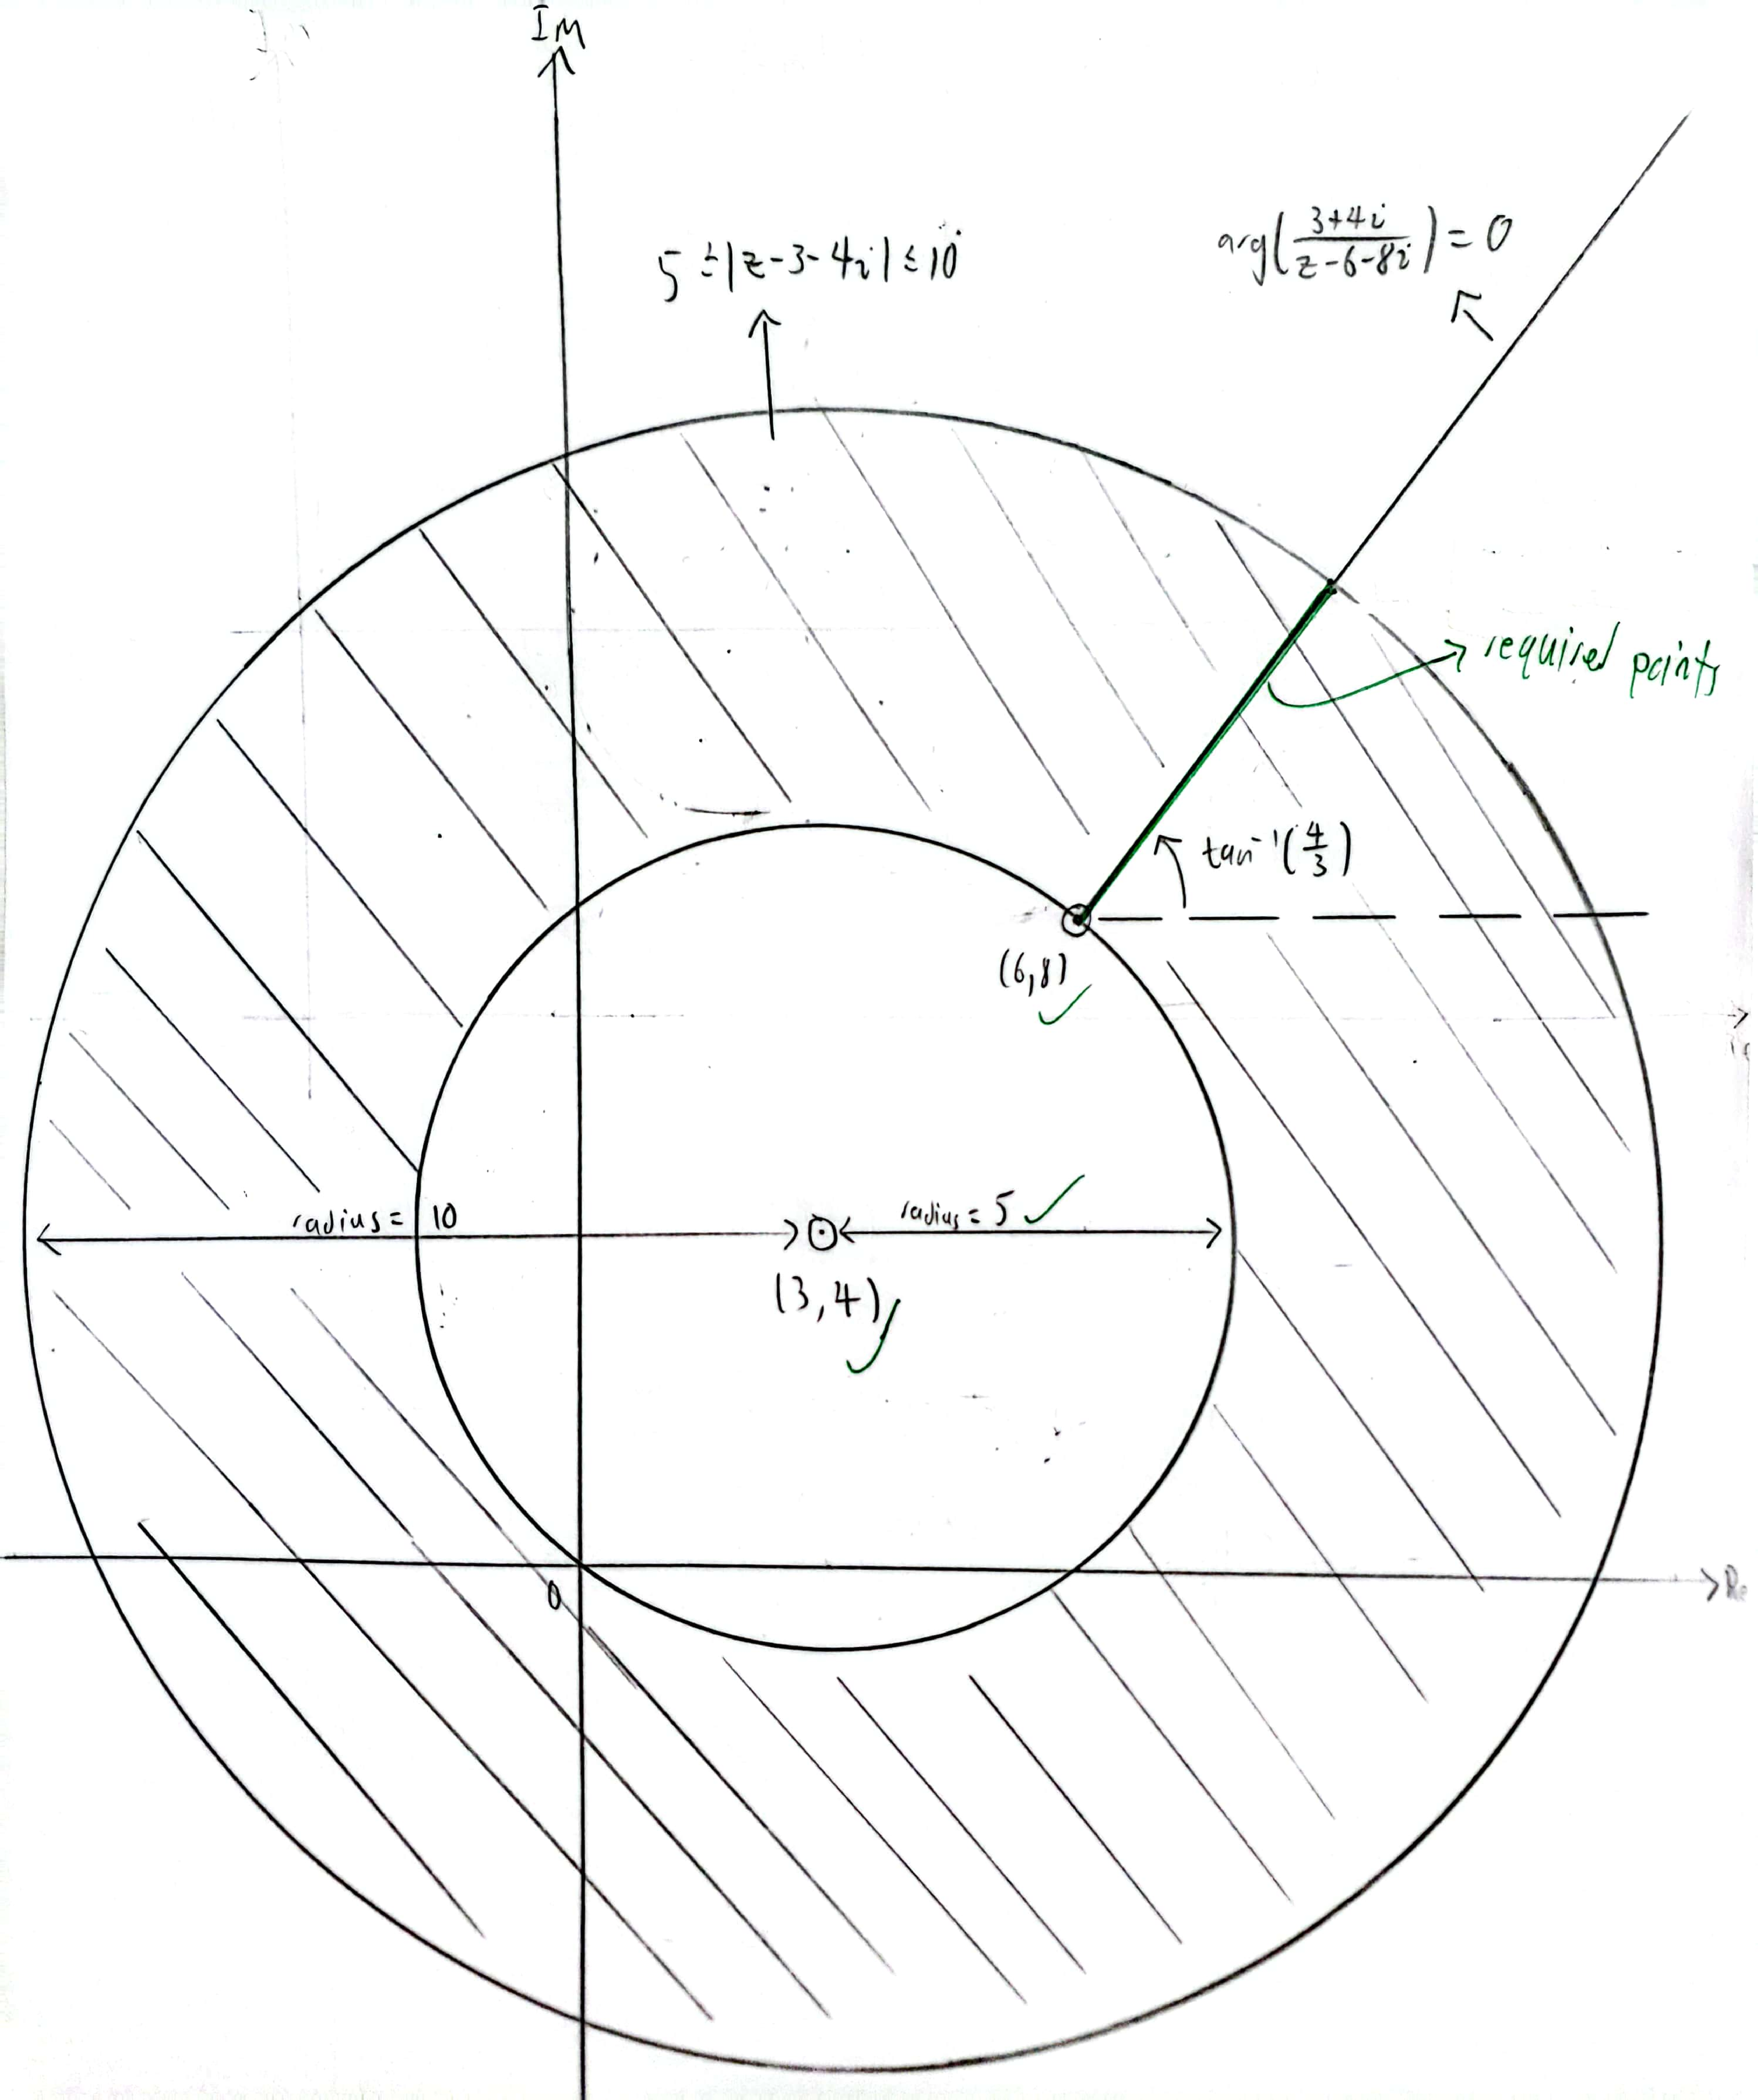
\includegraphics[width=0.6\textwidth,page=1]{../Diagrams/Complex-revision.pdf}
    \caption{\ref{Me} \textcolor{green!85!black}{Annotations} that improve clarity.}
    \label{fig:complex-clarity-improvements}
  \end{figure}
  \begin{figure}[H]
    \centering
    \begin{subfigure}[c]{0.45\textwidth}
      \centering
      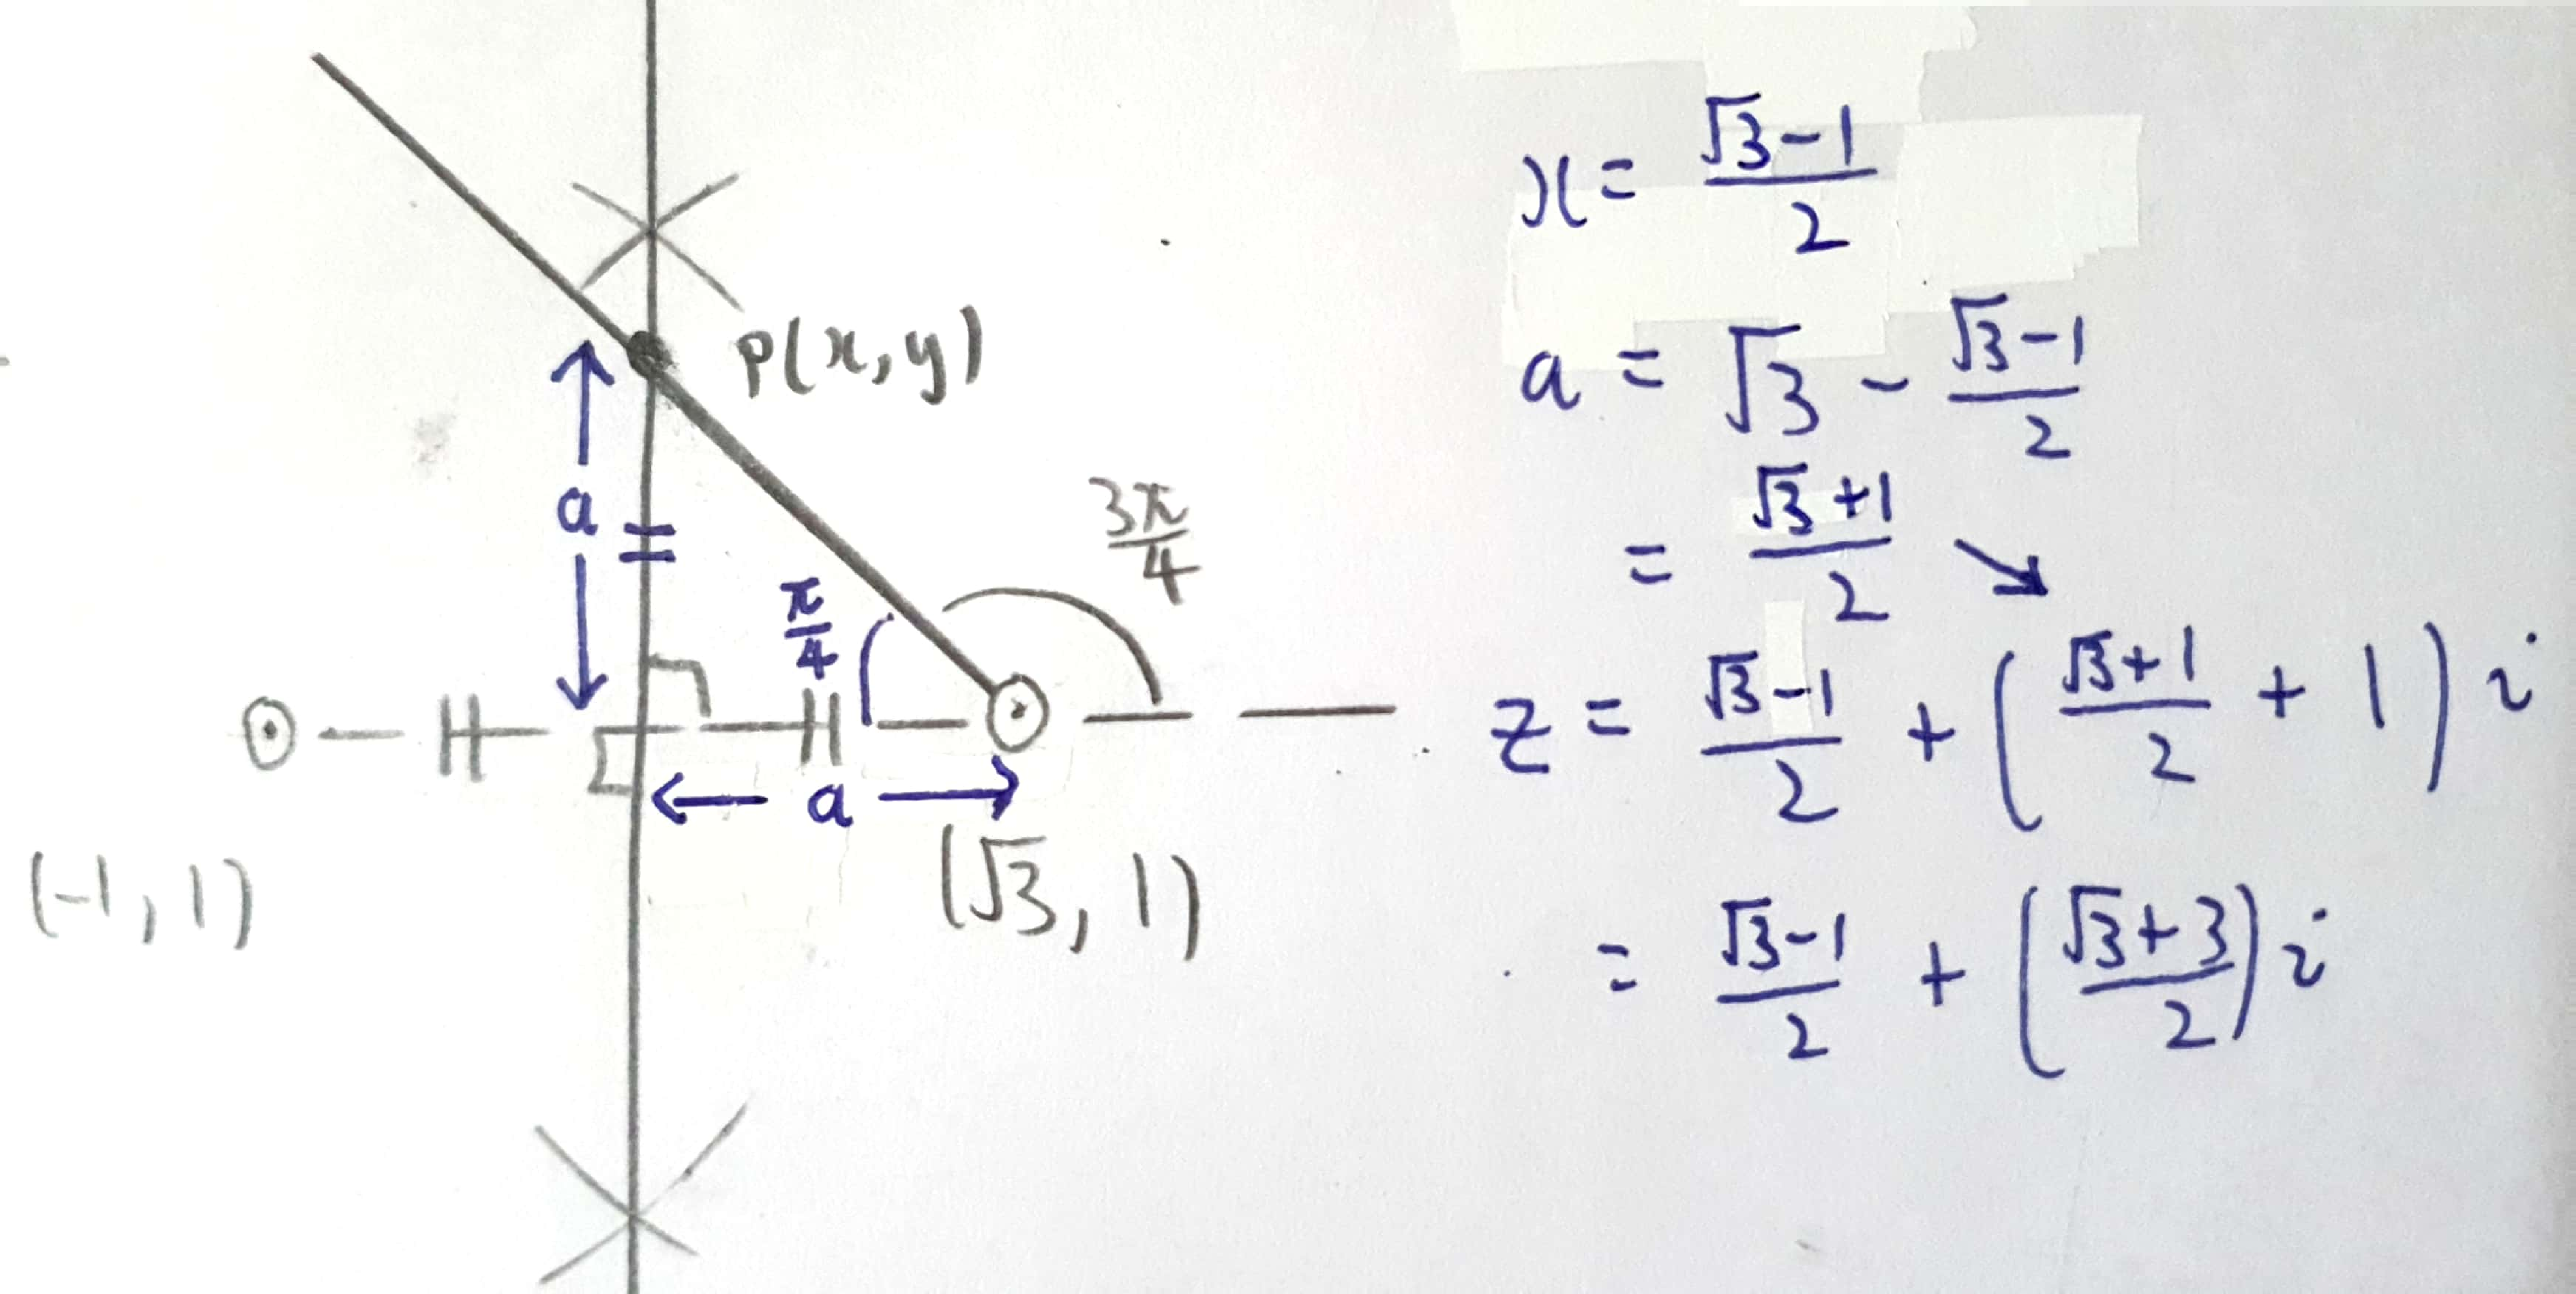
\includegraphics[width=\textwidth,page=1]{../Diagrams/FM-CT-2024-Q5.pdf}
      \caption{Finding the intersection of the two lines.}
  \end{subfigure}\hfill
  \begin{subfigure}[c]{0.45\textwidth}
      \centering
      \includegraphics[width=\textwidth,page=2]{../Diagrams/FM-CT-2024-Q5.pdf}
      \caption{Finding the radius \(R\) for which the circle just touches the half-line.}
  \end{subfigure}

  \begin{subfigure}[c]{0.45\textwidth}
    \centering
    \includegraphics[width=\textwidth,page=3]{../Diagrams/Complex-revision.pdf}
    \caption{Finding the shortest distance \(L\) and \(D\) of \((2,-\sqrt{3})\), from the circle and line, respectively.}
  \end{subfigure}
    \caption{\ref{Me} The \textcolor{blue}{writing in blue} denote the deductions we should make.}
    \label{fig:RVFM-CT-2024-Complex}
  \end{figure}
\end{example}